\begin{remark}
    Section made from lectures done by Dr.\ Emma Bland. Other sources are \citet{BrekkeAsgeir2013Potu} --- chapter 2 --- and \citet{NesseTyssoy2010Cium}.
\end{remark}
\section[Structure and dynamics of the atmosphere]{Structure and dynamics of the atmosphere (AB 2.1 \& 2.2)}
\begin{definition}[Atmosphere]\label{def:atmosphere}
    An atmosphere is the gaseous envelope around a celestial body, held in place by gravity. Stars, planets and large moons can sustain atmospheres, asteroids cannot.
\end{definition}
The presence of an atmosphere depends on gravity (attraction of particles), temperature (speed of particles) and composition (lighter particles move faster). For a stable atmosphere where
\begin{equation*}
    v_{\tn{thermal}}=\sqrt{\frac{2kT}{m}},\quad v_{\tn{escape}}=\sqrt{\frac{2GM}{r}}
\end{equation*}
you need that \(v_{\tn{thermal}}^2\ll v_{\tn{escape}}^2\) such that
\begin{equation*}
    kT\ll\frac{GMm}{r}
\end{equation*}
Hence, cold atmospheres and atmospheres with heavy constituents are more stable.
\subsection{The atmospheric layers}
The layers in the atmosphere ends with ``-sphere'' whilst the transition zones ends with ``-pause''. \Cref{fig:L6_atmos_layers} show the bottom layers and the transition zones with the corresponding heights at where they exist. The temperature profile changes a lot due to different sources at different heights, losses and transport. Sources of temperature is convection from the ground (troposphere), absorption of solar UV and X-ray (dissociation, ionization etc.\ give heat), energetic charged particles from the magnetosphere, Joule heating by ionospheric currents and dissipation of tidal and gravity waves. Losses are radiation, and mostly infrared, while transport can be radiation (mostly at the lowest levels), conduction (mostly thermosphere due to free electrons), convection (allows for heat transport from thermosphere to mesosphere), chemical transport (ionization in one place, recombination in another place) and horizontal transport due to winds.
\begin{figure}[t]
    \centering
    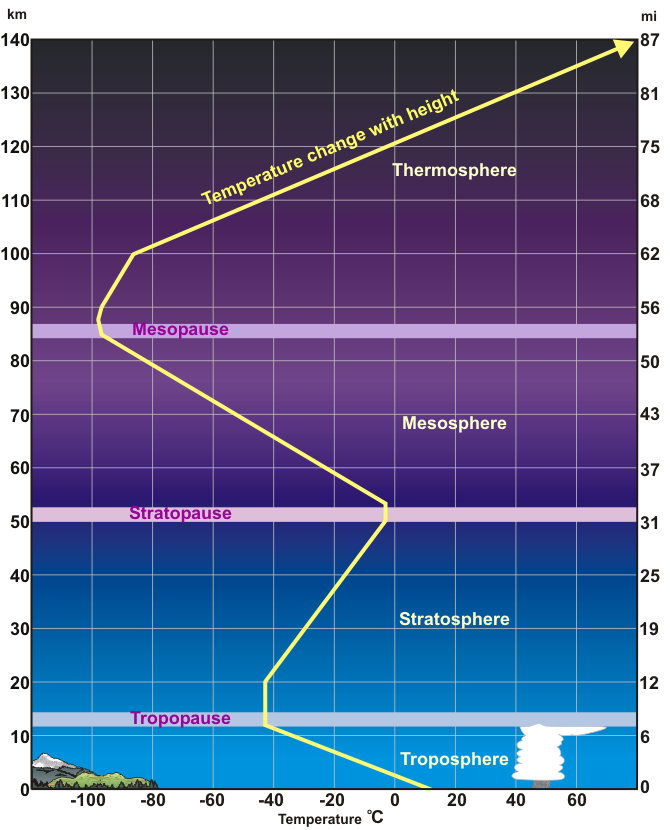
\includegraphics[width=.4\linewidth]{bilder/L6_atmos_layers.jpg}
    \caption{Layers in the atmosphere.}\label{fig:L6_atmos_layers}
\end{figure}

\subsection{Three cell global circulation pattern}
The three cell global circulation pattern is shown in \cref{fig:L6_three_cell_circulation}. The \emph{Hadley cell} can be found at \(0\)-\(\SI{30}{\degree}\). Here, air rises at equator resulting in that the upper air moves poleward. The Coriolis force then deflects the wind and it sinks at \(\pm\SI{30}{\degree}\). This process gives a belt of high surface pressure at \SI{30}{\degree}. The \emph{polar cell} can be found from \(60\)-\(\SI{90}{\degree}\). Cold, dense air descends at the pole which then cause high surface pressure. We get an equatorward flow near the surface, and deflection to the right due to Coriolis force. In between, from \(30\)-\(\SI{60}{\degree}\) we find the \emph{Ferrel cell}. The Ferrel cell is weak due to the lack of a strong heat source/sink, making air flows and temperatures highly variable.
\begin{figure}[t]
    \centering
    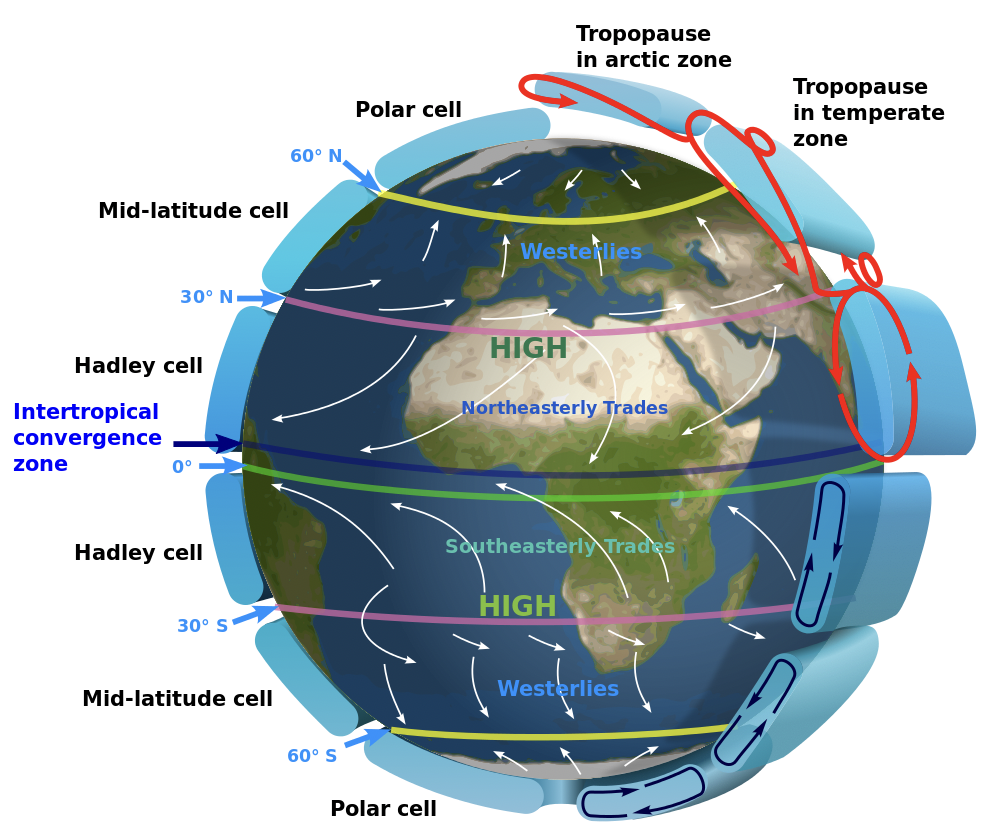
\includegraphics[width=.65\linewidth]{bilder/L6_three_cell_circulation.png}
    \caption{The three cell global circulation pattern.}\label{fig:L6_three_cell_circulation}
\end{figure}

\subsection{Stratospheric circulation}
\Cref{fig:L6_strat_circulation} show stratospheric circulation. The \emph{polar vortex} is a large area of low pressure (cyclone) formed in the upper troposphere and stratosphere. The pressure is stronger in the winter, and also stronger in the northern hemisphere. The \emph{polar night jet} lies on the border of the polar vortex. This is a strong westerly jet \(\sim \SI{100}{\metre/\second}\) centered around \SI{60}{\degree} latitude in the stratosphere and mesosphere during winter. It arises due to large temperature (and pressure) differences between equator and winter pole and the Coriolis effect. Warm air moves along the edge of the polar vortex, but cannot enter it. \emph{Summer easterlies} are zonal winds surrounding polar anticyclones in the stratosphere during summer. \emph{Stratospheric meridional circulation/Brewer-Dobson circulation} is meridional circulation from the tropics towards the poles in both hemispheres (stronger in winter) and this is driven by atmospheric waves. It is this circulation that is used to explain transport of ozone from tropical to polar latitudes. The last wind we consider is the \emph{quasi-biennial oscillation} (QBO). This has a 28--29-month cycle in zonal wind direction (between westerly and easterly) in the equatorial stratosphere, and it will mostly be within \SI{15}{\degree} latitude in each hemisphere.
\begin{figure}[t]
    \centering
    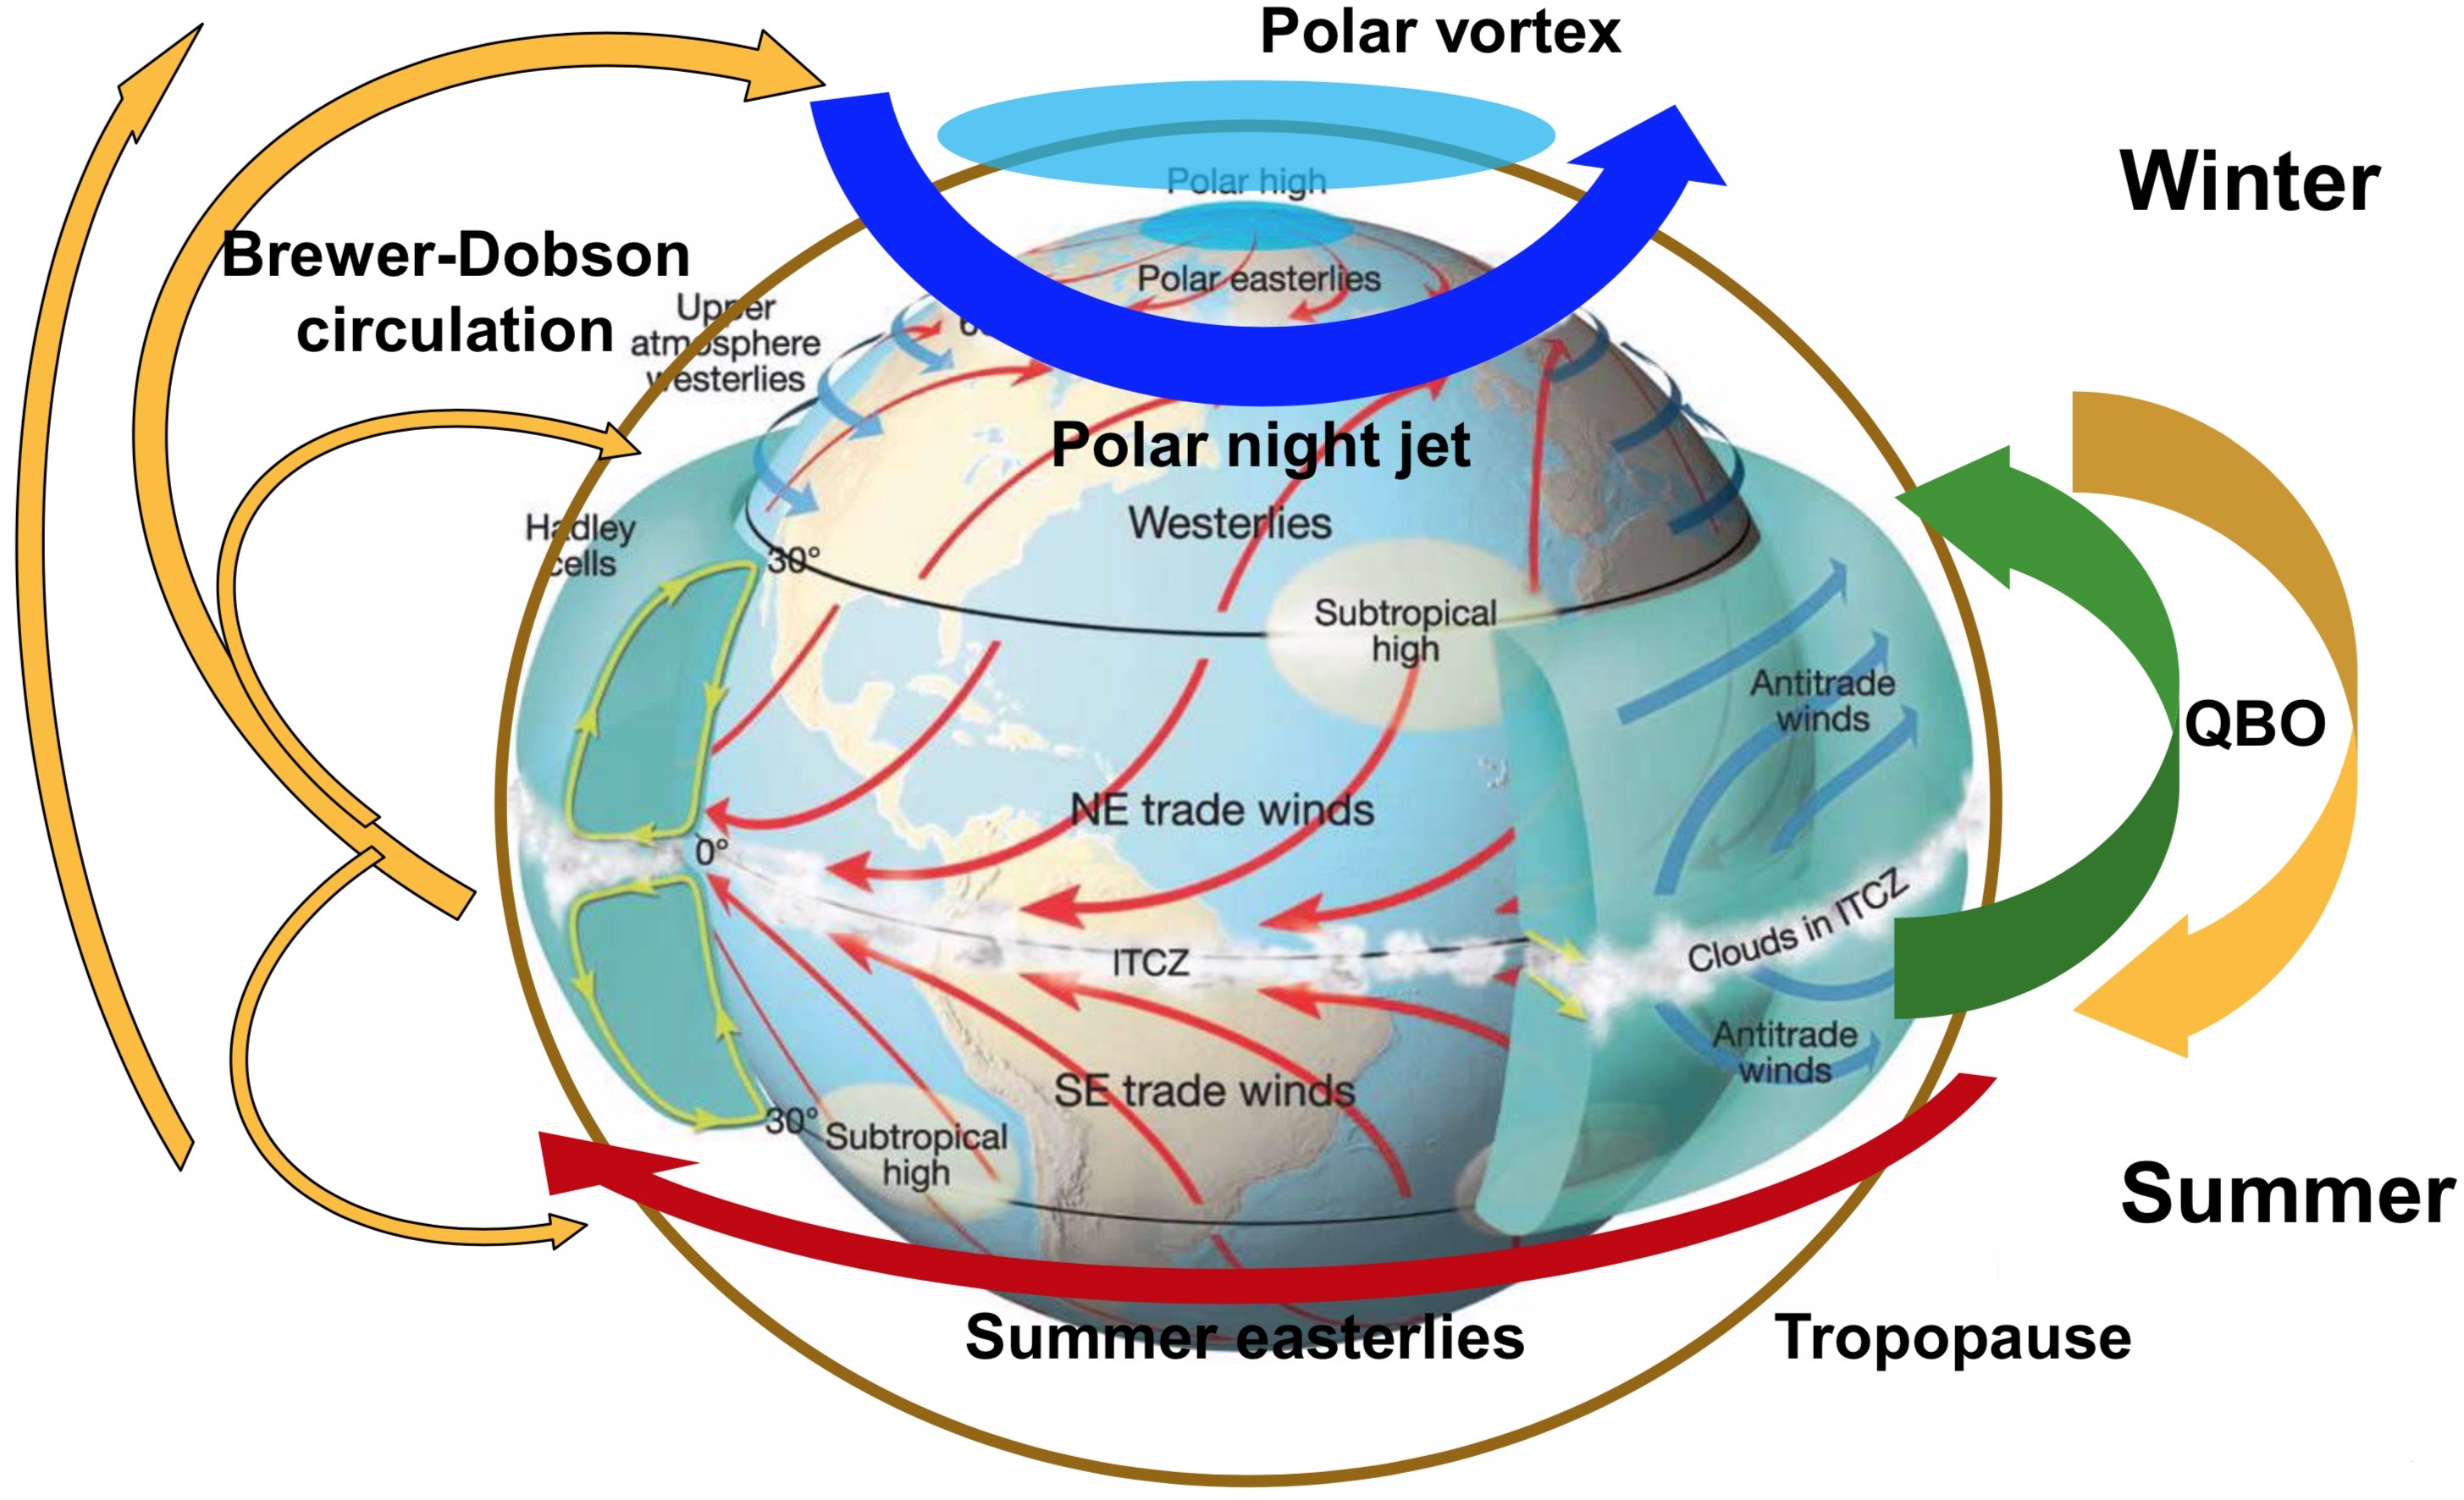
\includegraphics[width=.7\linewidth]{bilder/L6_strat_circulation.jpg}
    \caption{The stratospheric circulation pattern.}\label{fig:L6_strat_circulation}
\end{figure}

\subsection{Basic dynamics: waves}
We may classify waves by horizontal scale size, one being of planetary size (\(10^7\si{\metre}\)), e.g.\ Rossby waves and the other being of synoptic scale (\(10^6\si{\metre}\)), e.g.\ gravity waves.

Gravity wave breaking happen when GWs propagate upward in the layers. The amplitude grows and is proportional to \(\rho^{-1/2}\). At some altitude the amplitude becomes so large that non-linear effects become important and the mean flow can no longer support wave propagation. Wave breaking impacts on zonal mean winds and temperatures, and it drives the inter-hemisphere meridional circulation in the mesosphere (summer to winter hemisphere).

\section[Energetic particle precipitation \& the neutral atmosphere]{Effects of energetic particle precipitation on the neutral atmosphere \citep{NesseTyssoy2010Cium}}
\subsection{Ionization sources}
Sources for ionization are cosmic radiation, solar proton events (come in on open field lines, noticed in polar cap), auroral precipitation and relativistic electrons. \Cref{fig:L6_ionization_sources} show the ionization sources in the atmosphere.
\begin{figure}[t]
    \centering
    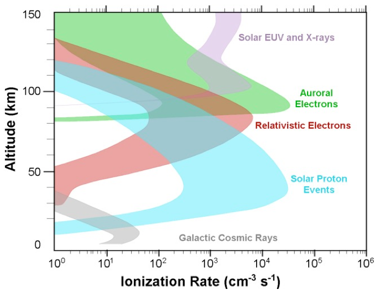
\includegraphics[width=.6\linewidth]{bilder/L6_ionization_sources.png}
    \caption{Ionization sources.}\label{fig:L6_ionization_sources}
\end{figure}

\subsubsection{Solar proton event}
\Cref{fig:L6_solar_proton_event} show how the proton flux changed during a solar proton event. From these events we get strong enhancement in energetic proton flux (\(>\SI{10}{\mega\electronvolt}\)), and damage to satellite electronics, radiation risk to astronauts and aircraft passengers/crew and HF radio wave absorption are among the effects we get from them, but they occur rarely (approx. 20/year at solar maximum, 0--3/year at solar min.). The events impact the whole polar cap and goes as far down as to the stratosphere. The effects it has on the atmosphere is well understood, and we have information about the flux. A proton flux measured by GOES-15, 1--16 September 2017 shows large enhancements in flux of high energy protons, and at Longyearbyen early on 5 September 2017 one could see loss of SuperDARN radar backscatter. At \url{https://umbra.nascom.nasa.gov/SEP/} you can find a list of such events.
\begin{figure}[t]
    \centering
    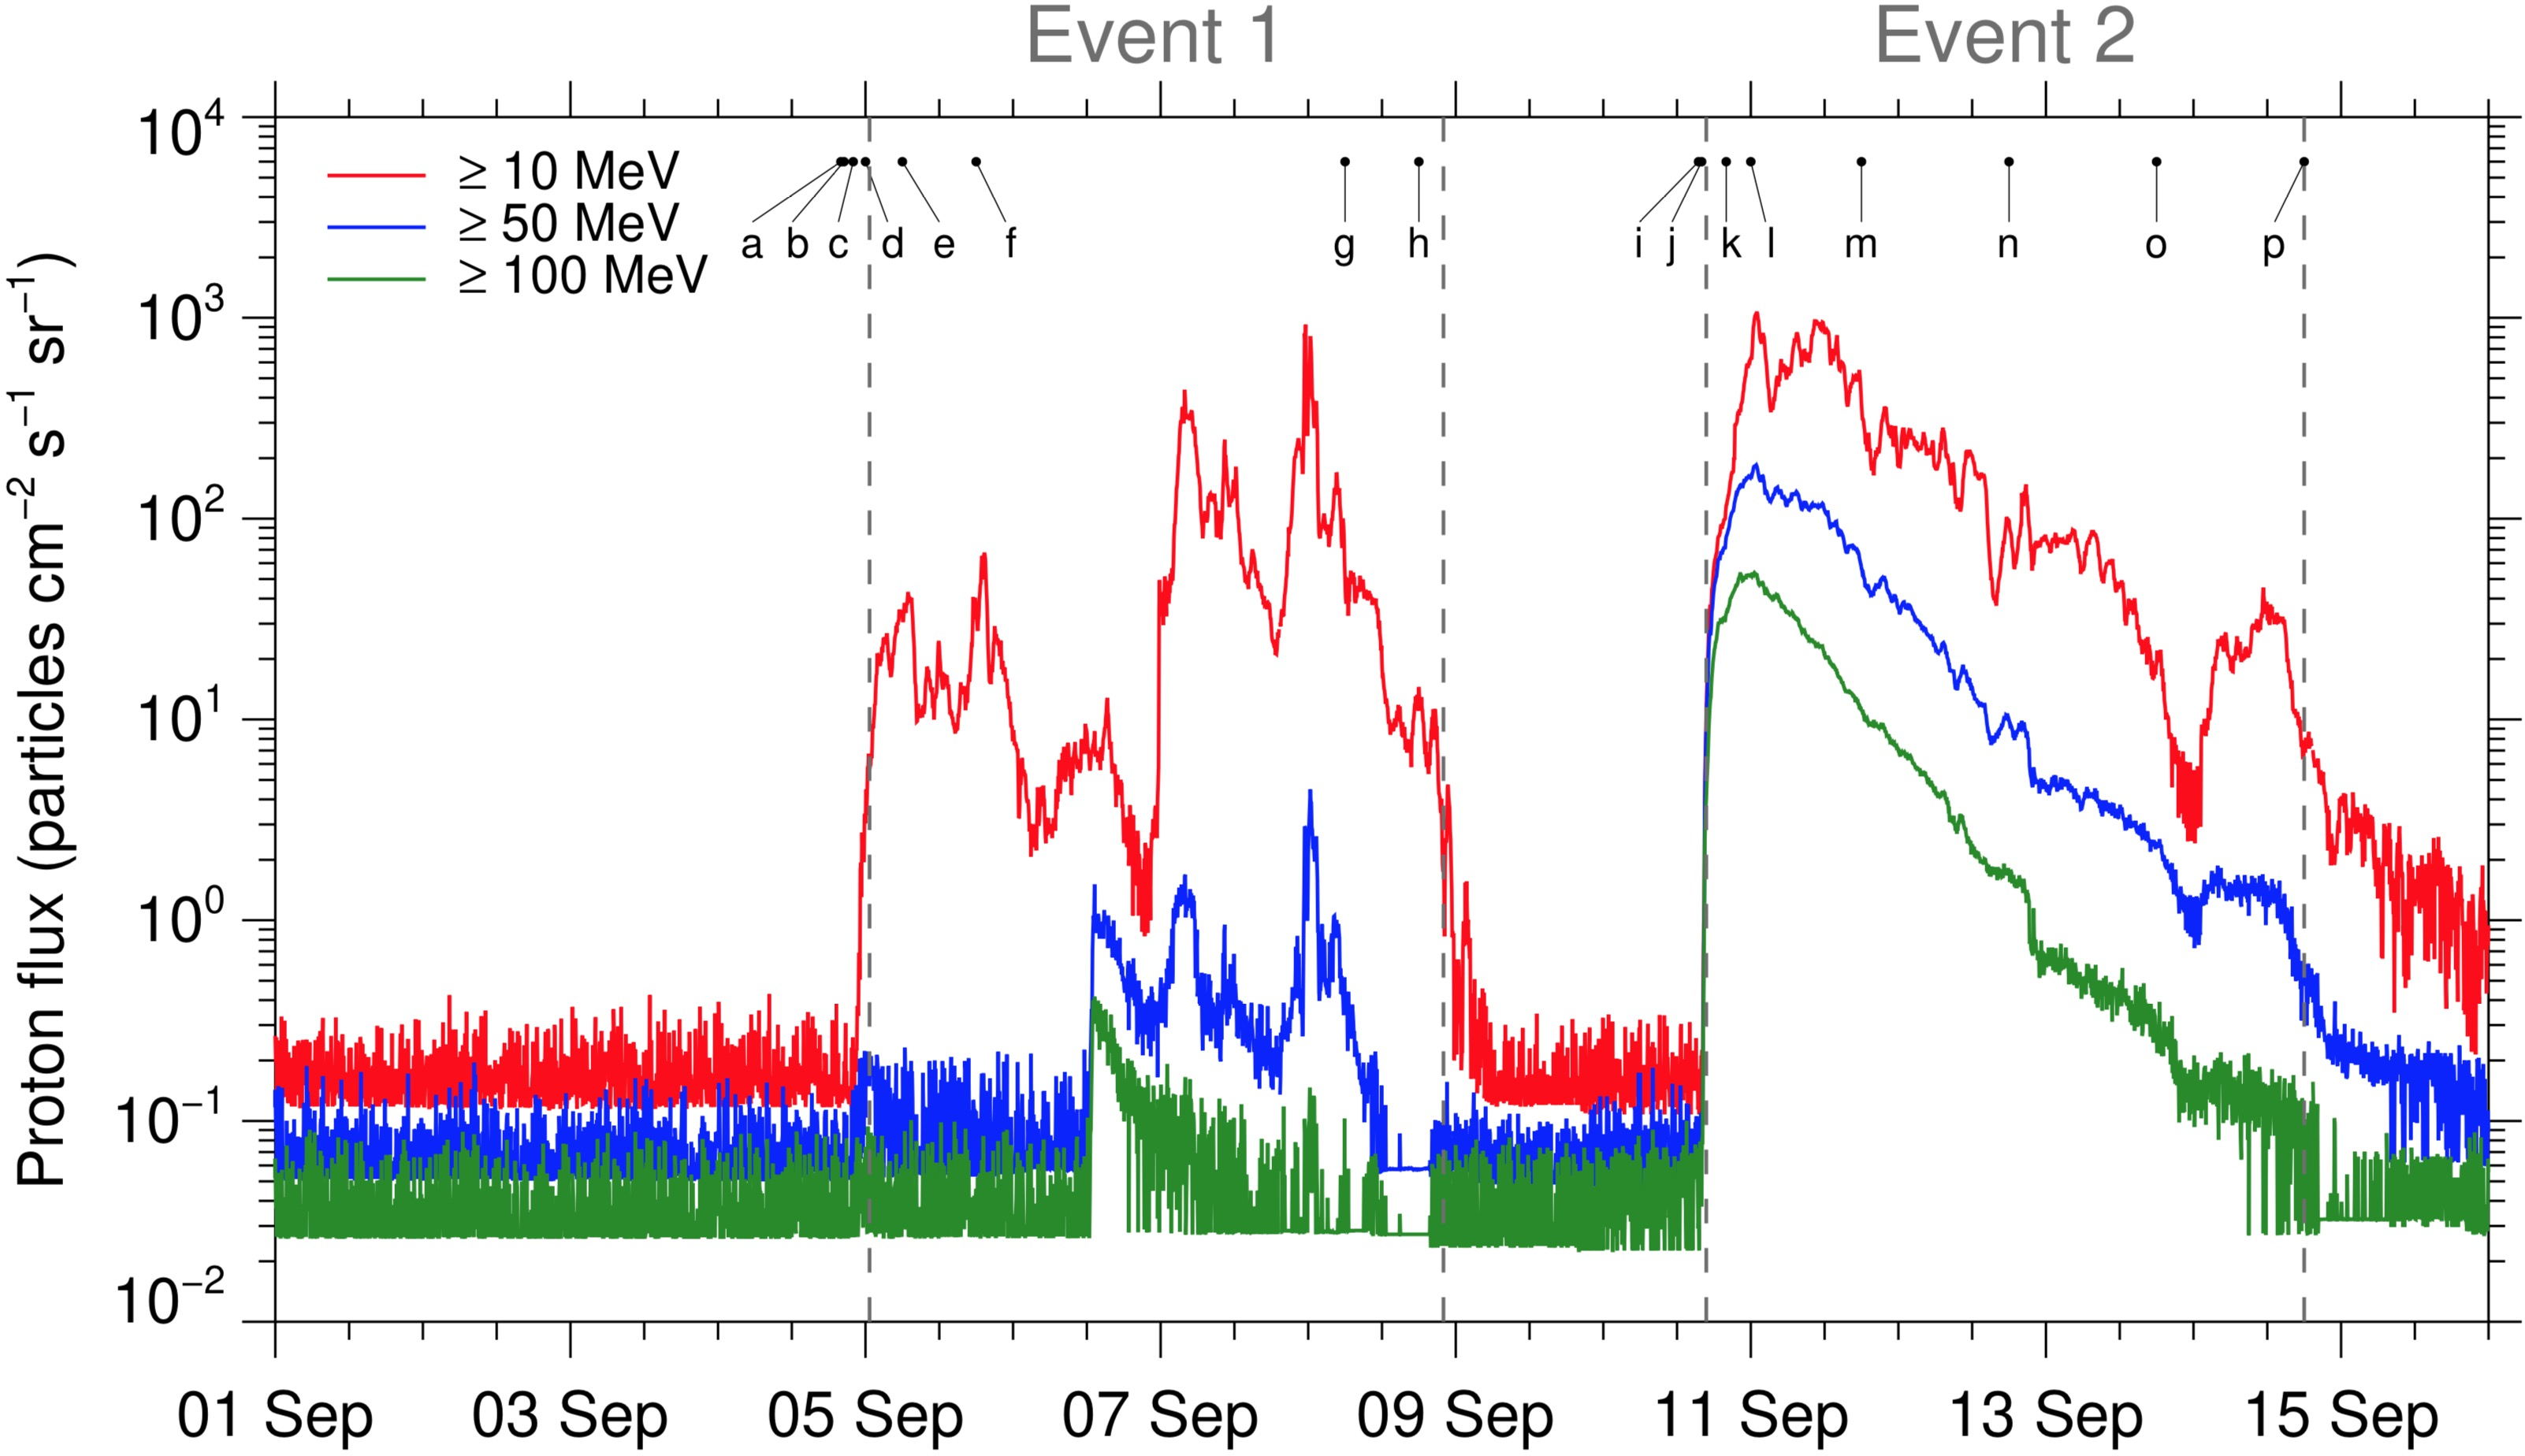
\includegraphics[width=.8\linewidth]{bilder/L6_solar_proton_event.jpg}
    \caption{Proton flux measured by GOES-15, 1--16 September 2017.}\label{fig:L6_solar_proton_event}
\end{figure}

\subsubsection{Electron precipitation}
Electron precipitation might give us relativistic electrons (\(\sim\SI{0.1}{\mega\electronvolt}\) to several \si{\mega\electronvolt}) during substorms and geomagnetic storms. When this is happening, we get auroral precipitation, including pulsating aurora. Compared to a solar proton event, electron precipitation is happening almost all the time, but impacts only the auroral oval.We do not have continuous observations of it and the effects on the atmosphere are not well understood. Auroral to relativistic energies are from \si{\kilo\electronvolt} to \si{\mega\electronvolt}, with pulsating aurora at keV level (electron precipitation).

The solar protons and the radiation belt electrons are a major source of ionization in the middle atmosphere.

The particle energy will determine the impact altitude. To produce \( 1 \) ion pair \si{\centi\metre^{-3}\second^{-1}} at \SI{60}{\kilo\metre} altitude (see \cref{fig:L6_impact_altitude}) we need
\begin{equation*}
    1\times\SI{20}{\mega\electronvolt}\tn{ protons } \si{\centi\metre^{-2}\second^{-1}}\quad\tn{or}\quad 100\times\SI{1}{\mega\electronvolt}\tn{ protons } \si{\centi\metre^{-2}\second^{-1}}
\end{equation*}
\begin{figure}[t]
    \centering
    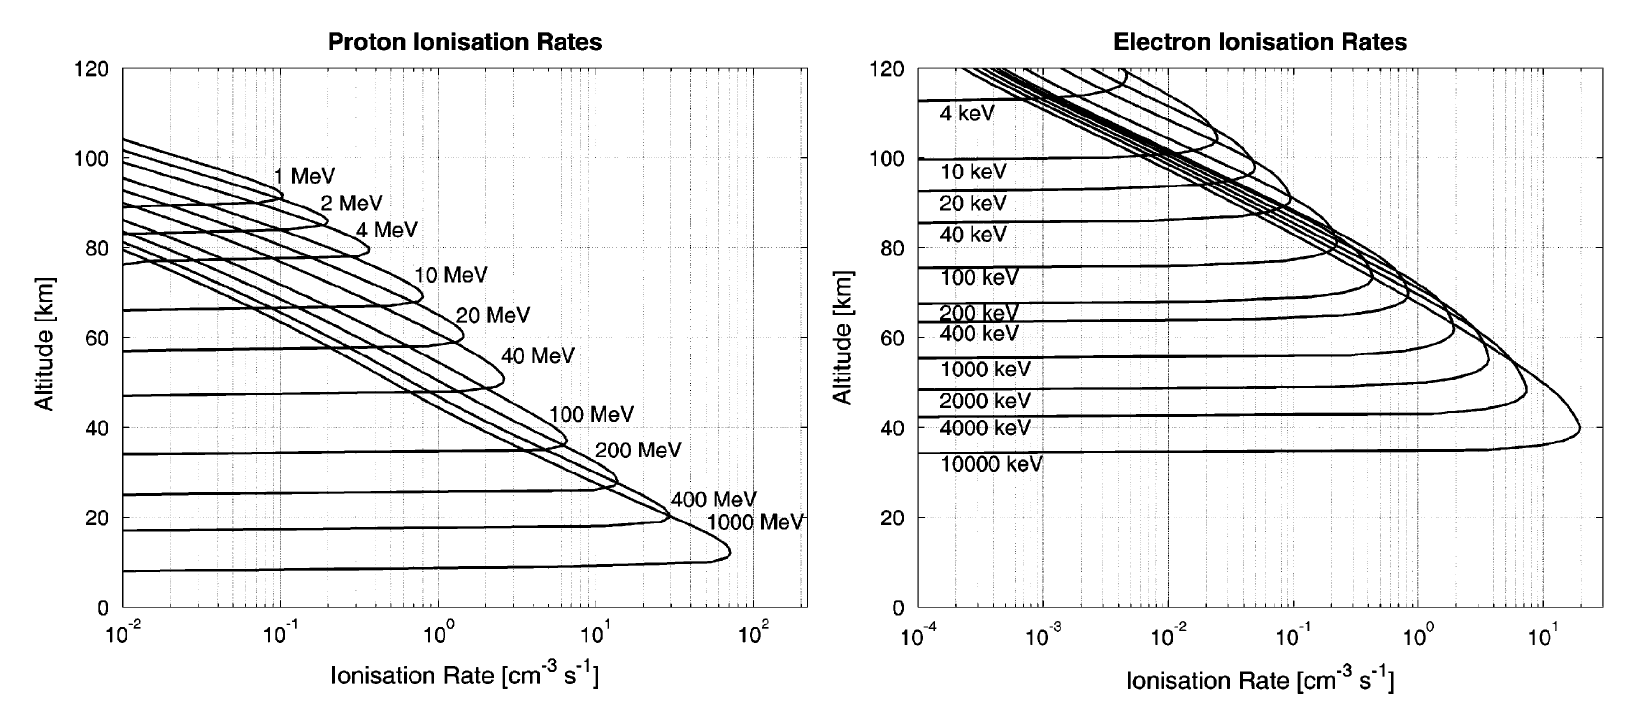
\includegraphics[width=.8\linewidth]{bilder/L6_impact_altitude.png}
    \caption{Altitude versus ionization rates for monoenergetic beams of protons (left) and electrons (right) \citep{TurunenEsa2009Iode}.}\label{fig:L6_impact_altitude}
\end{figure}
E-region ions are produced primarily by photoionization of molecular nitrogen and oxygen by UV radiation and X-rays, \(n_e\approx n_{\tn{O}_2^+}+n_{\tn{NO}^+}\). Positive ions in the D-region consists of a number of heavy cluster ions, e.g.~\(\tn{NO}^+\) and \(\tn{O}_2\). Negative ions in the D-region are density dependent, there is photo detachment, collisional detachment and ion-ion recombination.

But the chemically reactive ions have implications for the neutral atmosphere composition. Formation of \(\tn{HO}_{\tn{X}}\) and \(\tn{NO}_{\tn{X}}\) by positive ion chemistry give the possibility that they catalyze the ozone destruction. \(\tn{HO}_{\tn{X}}\) (\(\tn{H}+\tn{OH}+\tn{HO}_2\)) have a short lifetime while \(\tn{NO}_{\tn{X}}\) (\(\tn{N}+\tn{NO}+\tn{NO}_2\)) have longer chemical lifetime in the dark, hence especially in the winter period. Ozone is important for the energy budget through its role as a solar radiation absorber and radiator. \(\tn{HO}_{\tn{X}}\) contribute to a rapid but short-lived ozone loss in the mesosphere, while the \(\tn{NO}_{\tn{X}}\) could potentially influence both the mesospheric and stratospheric ozone balance.
\begin{align*}
    \tn{X}+\tn{O}_3&\rightarrow \tn{XO}+\tn{O}_2\\
    \tn{XO}+\tn{O}&\rightarrow \tn{X}+\tn{O}_2\\
    \tn{Net:}~\tn{O}+\tn{O}_3&\rightarrow 2\tn{O}_2
\end{align*}
Vertical downward transport is therefore mostly due to \(\tn{NO}_{\tn{X}}\), and also largely determined by the polar vortex.

\subsection{Consequences for atmospheric dynamics}
Chemical changes couple to wind and temperature changes and affect the energy transfer in the atmosphere. Energetic particle precipitation produces \(\tn{HO}_\tn{X}\) and \(\tn{NO}_\tn{X}\) which are catalysts for ozone destruction. More or less ozone give heating and cooling, i.e.\ temperature changes. This will then give winds which also has an impact on atmospheric waves (energy transfer). We then see that we have a dynamical amplification of initial impact. So we go from energetic particle precipitation (EPP) to increased winds in an indirect way (but not that long).

\section[Collisions between ions \& neutral particles]{Collisions between ions \& neutral particles (AB 2.13)}
Consider a gas consisting of two species, \(m\) and \(n\). These particles undergo collisions. Assume that the force per unit mass acting on the \(m\)-type particles due to collisions with \(n\)-type particles is proportional to the velocity difference between the two species, \(f_{m,n}\propto\gf{u}_m-\gf{u}_n\), with the force being given as
\begin{equation*}
    f_{m,n}=-\nu_{mn}\left(\gf{u}_m-\gf{u}_n\right)=\fracd{\gf{u}_m}
\end{equation*}
where \(f_{m,n}\) is the force (per unit mass) reducing \(\gf{u}_m\) due to collisions with \(n\)-type particle (\(u_m>u_n\)) and \(\nu_{mn}\) is the collision frequency. Momentum must be conserved, so
\begin{equation*}
    \rho_{m}f_{m,n}+\rho_{n}f_{n,m}=0
\end{equation*}
\coloredeq{eq:L6_collision_freq}{\therefore\rho_m\nu_{mn}\left(\gf{u}_m-\gf{u}_n\right)+\rho_n\nu_{nm}\left(\gf{u}_n-\gf{u}_m\right)=0}
So we can see that \(\rho_m\nu_{mn}=\rho_n\nu_{nm}\). For simplicity, consider only 1-dimensional motion. The equation of motion for \(m\)-type particles can be written as
\begin{equation*}
    \frac{\tn{d}u_m}{u_m-u_n}=-\nu_{mn}\tn{d}t
\end{equation*}
Using separation of variables we see, after integration, that this equation has the solution
\begin{equation*}
    u_m=u_m^0e^{-\nu_{mn}t}+u_n\left(1-e^{-\nu_{mn}t}\right)
\end{equation*}
where \(u_m\equiv u_m^0\) at \(t=0\). We get that \(\lim_{t\rightarrow\infty}u_m=u_n\) (equilibrium sol.\ for \(u_m\)). This occurs with characteristic relaxation time \(\tau_{m,n}=\frac{1}{\nu_{mn}}\). We can also write the equation of motion for \(n\)-type particles
\begin{equation*}
    u_n=u_n^0e^{-\nu_{nm}t}+u_m\left(1-e^{-\nu_{nm}t}\right)
\end{equation*}
with relaxation time
\begin{equation*}
    \tau_{nm}=\frac{1}{\nu_{nm}}=\frac{\rho_n}{\rho_m\nu_{mn}}=\frac{\rho_n}{\rho_m}\tau_{mn}
\end{equation*}
by using \cref{eq:L6_collision_freq}. What happens if \(\rho_m\gg\rho_n\)? Well, we have \(\tau_{mn}\gg\tau_{nm}\). This means that the \(n\)-type particles will reach equilibrium velocity \(\gf{u}_m\) much more quickly than the \(m\)-type particles will reach \(\gf{u}_n\). It also means that the \(n\)-type particles will ``feel'' the presence of the \(m\)-type particles more than the \(m\)-type will ``feel'' the \(n\)-type. I.e.\ we have \emph{drag} from one kind of particle to another.

The mean velocity is defined as
\begin{equation*}
    \widetilde{\gf{u}}:=\frac{\rho_{mn}\gf{u}_m+\rho_n\gf{u}_n}{\rho}
\end{equation*}
where \(\rho=\rho_m+\rho_n\). Since \(\fracd{\rho}=0\), we can write the momentum equation as
\begin{equation*}
    \rho\fracd{\widetilde{\gf{u}}}=-\left[\rho_m\nu_{mn}\left(\gf{u}_m-\gf{u}_n\right)+\rho_n\nu_{nm}\left(\gf{u}_n-\gf{u}_m\right)\right]=0
\end{equation*}
so the mean velocity is constant!
\begin{equation*}
    \gf{u}(\infty)=\gf{u}(t)=\gf{u}(0)
\end{equation*}

\section[Drag effects]{Drag effects (AB 2.15)}
Consider a simplified ionosphere with one neutral species and one ion species. These particles have velocities
\begin{equation*}
    \underset{\substack{\uparrow \\ \tn{ion}}}{\gf{v}_i}\quad\tn{and}\quad\underset{\substack{\uparrow \\\tn{neutral}}}{\gf{u}_n}
\end{equation*}
Assume that the neutral gas is in hydrostatic equilibrium, i.e.\ ignore vertical motion of neutrals. We consider three different cases. \boxed{\tn{Case 1}} (\Cref{fig:L6_no_init_neut_wind}). We here assume \(\gf{u}_{n0}=0\), i.e.\ no neutral wind and that the electric field is applied perpendicular to \(B\) so that
\begin{equation*}
    \gf{v}_{i0}=\frac{\gf{E}\times\gf{B}}{B^2}
\end{equation*}
The horizontal component of ion velocity will drag the neutrals along. Neutrals will also drag ions along which in turn does so \(\gf{v}_i\) will gain a component \(\vert\vert \) to \(\gf{B}\). We then get a stationary state when the ions and neutrals are moving horizontally at the same speed.
\begin{equation*}
    u_n=\frac{v_{i0}}{\sin(I)}=\frac{1}{\sin(I)}\frac{E}{B}
\end{equation*}
\boxed{\tn{Case 2}} (\Cref{fig:L6_no_init_ion_wind}). We now assume that \(\gf{v}_{i0}=0\), i.e.\ that ions initially are at rest meaning no \(E\)-field, and that we have horizontal neutral wind in the southward direction. The component of \(\gf{u}_n\) \(\vert\vert \) to \(\gf{B}\) will generate ion motion \(\vert\vert \) to \(\gf{B}\). The steady state ion velocity \(\gf{v}_i\) along the field is then given as
\begin{equation*}
    v_i=u_{n0}\cos(I)
\end{equation*}
or as
\begin{align*}
    &\tn{Horizontal component: } \hspace{-3cm}&v_{iH}&=u_{n0}\cos^2I&\\
    &\tn{Vertical component: } \hspace{-3cm}&v_{iV}&=u_{n0}\cos(I)\sin(I)&
\end{align*}
\boxed{\tn{Case 3}} (\Cref{fig:L6_diffusion_wind}). In our last case we again consider no initial neutral wind, \(u_{n0}=0\), and that plasma is diffusing downwards along the \(B\)-field lines at velocity \(v_{iD}\) (diffusion due to gravity + \(\nabla P\)). The ion motion has a horizontal component
\begin{equation*}
    v_{iH}=v_{iD}\cos(I)
\end{equation*}
This will drag the neutrals along until they attain horizontal velocity \(\gf{u}_n\). \(\gf{u}_n\) will produce an additional ion velocity along the field line, \(u_n\cos(I)\), and we get equilibrium when
\begin{align*}
    u_n=\left(v_{iD}+u_n\cos(I)\right)\cos(I)\\
    \Rightarrow u_n=\frac{v_{iD}\cos(I)}{\sin^2(I)}
\end{align*}
The final plasma velocity \(\vert\vert \) to \(B\) is
\begin{equation*}
    v_i=\frac{v_{iD}}{\sin^2(I)}
\end{equation*}
\begin{figure}[t]
    \centering

    \begin{subfigure}[t]{.32\linewidth}
        \centering
        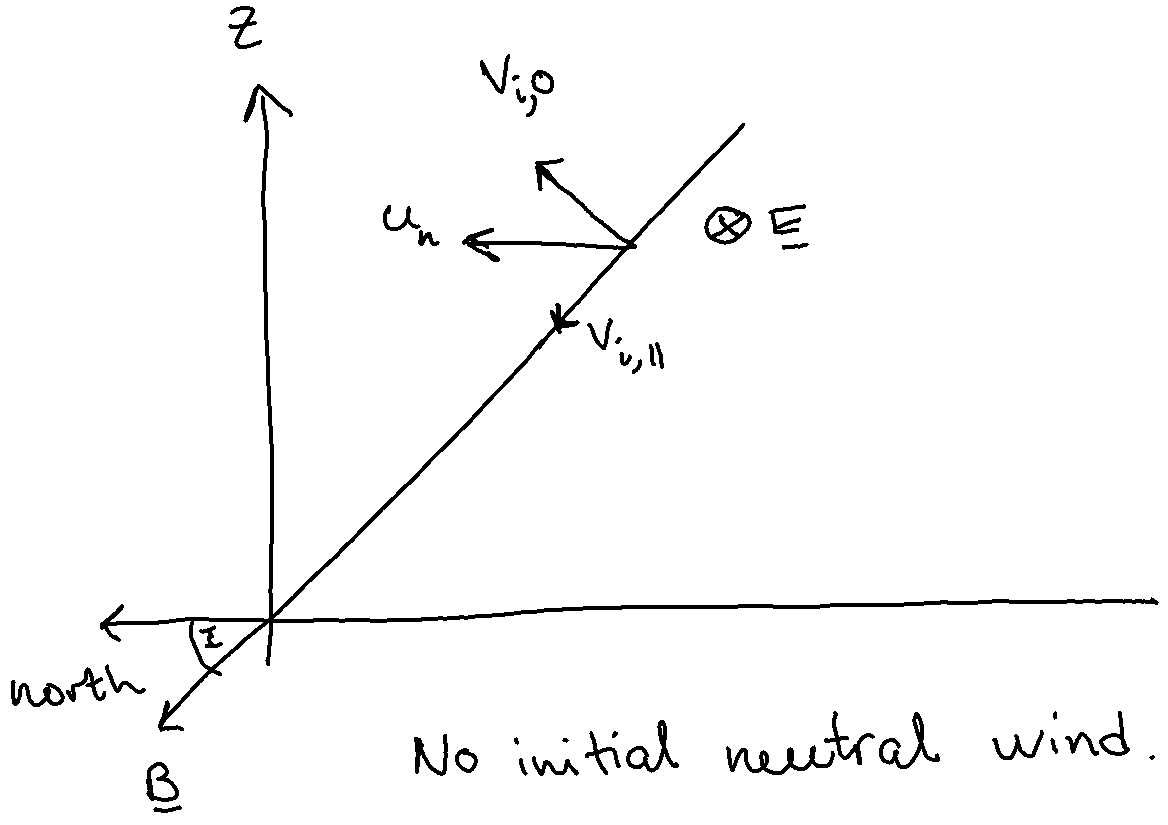
\includegraphics[width=\linewidth]{bilder/L6_no_init_neut_wind.png}
        \caption{}\label{fig:L6_no_init_neut_wind}
    \end{subfigure}
    \begin{subfigure}[t]{.32\linewidth}
        \centering
        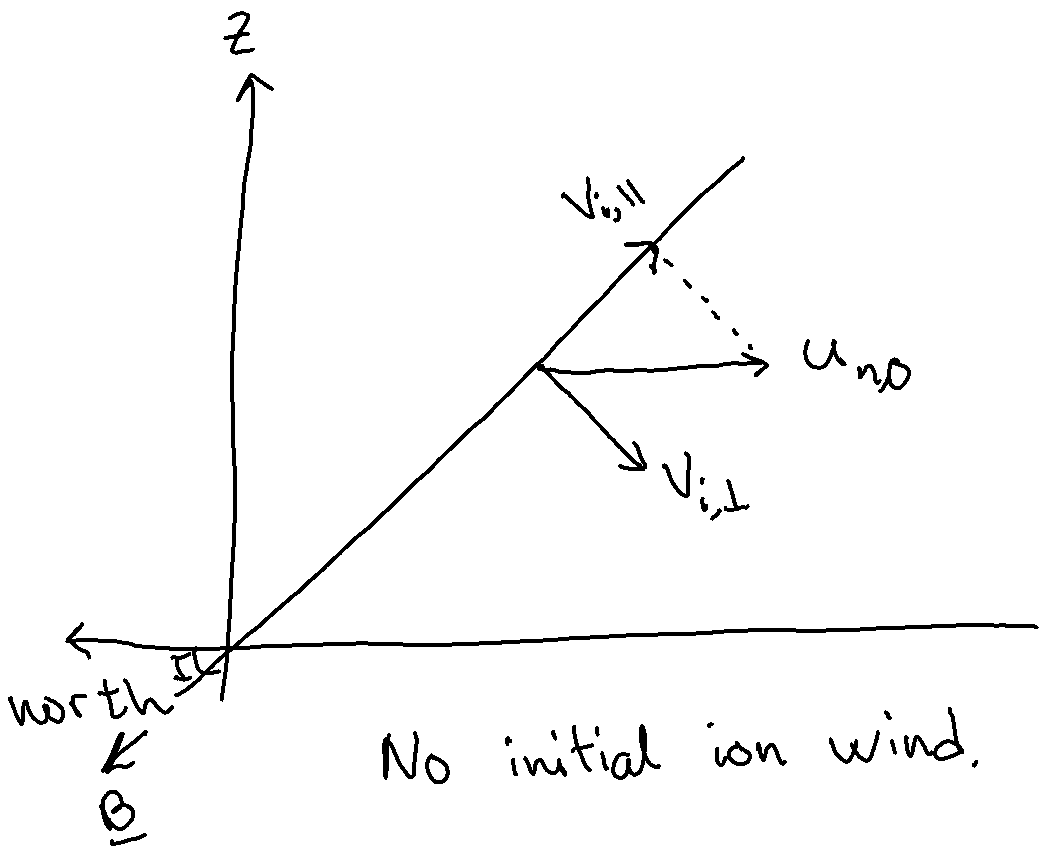
\includegraphics[width=\linewidth]{bilder/L6_no_init_ion_wind.png}
        \caption{}\label{fig:L6_no_init_ion_wind}
    \end{subfigure}
    \begin{subfigure}[t]{.32\linewidth}
        \centering
        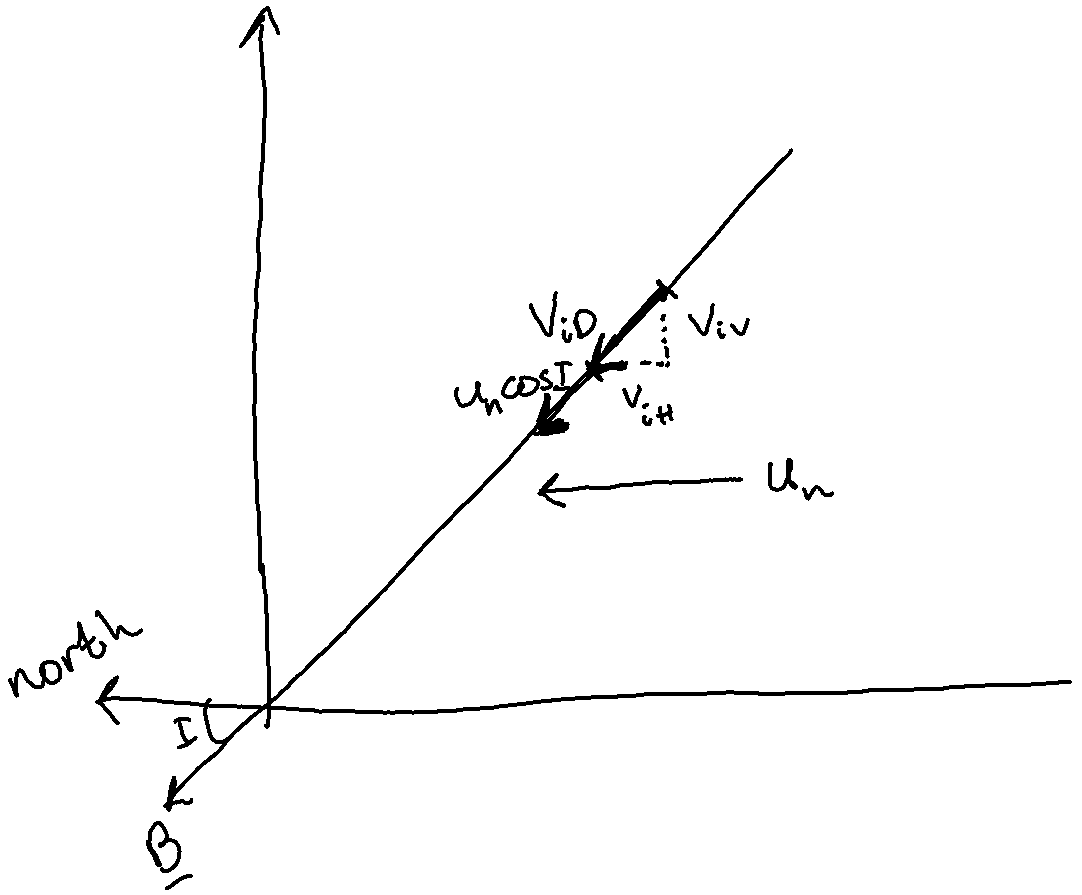
\includegraphics[width=\linewidth]{bilder/L6_diffusion_wind.png}
        \caption{}\label{fig:L6_diffusion_wind}
    \end{subfigure}

    \caption{\subref{fig:L6_no_init_neut_wind}: No initial neutral wind. \subref{fig:L6_no_init_ion_wind}: No initial ion wind. \subref{fig:L6_diffusion_wind}: Diffusion effect on ion wind.}\label{fig:L6_ion_and_neutral_winds}
\end{figure}

\section[Thermospheric neutral wind]{Thermospheric neutral wind (AB 2.16, 2.17 \& 2.18)}
During daytime, we get an expansion of the atmosphere called the diurnal bulge. The temperature distribution creates large-scale pressure gradients which again creates winds. In general we get velocities directed from the dayside across the pole to the nightside and the wind speeds can be of \(\sim\SI{40}{\metre\second^{-1}}\) directed approximately perpendicular to the isotherms
\begin{figure}[t]
    \centering
    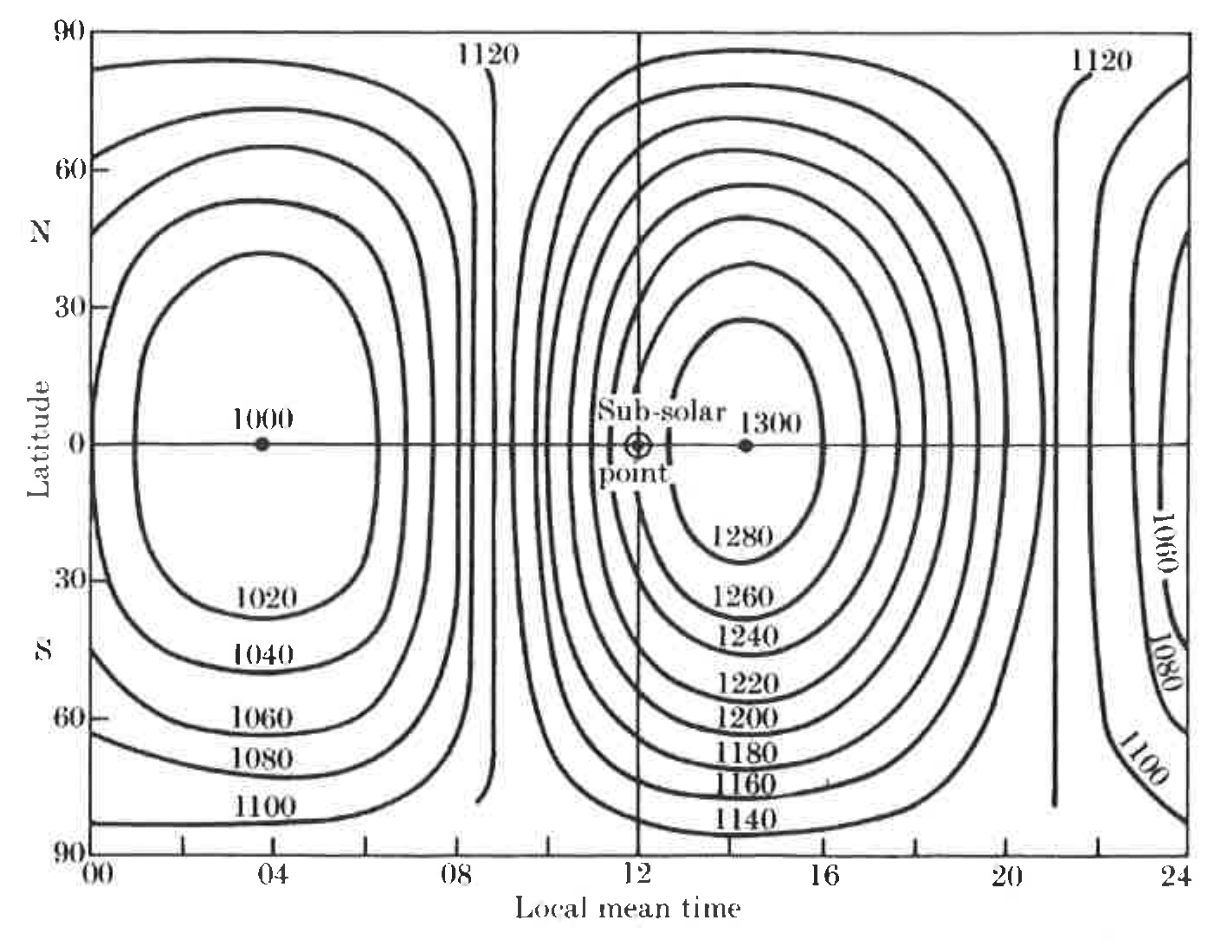
\includegraphics[width=.6\linewidth]{bilder/L6_winds_diurnal.png}
    \caption{Modelled isotherms at the thermopause, \(\sim\SI{400}{\kilo\metre}\) altitude.}\label{fig:L6_winds_diurnal}
\end{figure}
The equation of motion for a neutral gas can be expressed as
\begin{equation*}
    \fracd{\gf{u}}=-\frac{1}{\rho}\nabla p+\gf{g}+\gf{f}
\end{equation*}
We ignore all terms except the pressure gradient force and \(\gf{f}\). A steady state solution for the neutral wind is
\begin{equation*}
    \gf{f}=\frac{1}{\rho}\nabla p
\end{equation*}
If we assume \(\gf{f}\) to only be caused by collisions between neutrals and ions (\(\gf{f}=-\nu_{ni}(\gf{u}_n-\gf{v}_i)\)) and that we have an ideal gas, the velocities will be
\begin{equation*}
    \gf{u}_n=-\frac{1}{\rho\nu_{ni}}\nabla p+\gf{v}_i=-\frac{k}{\rho\nu_{ni}}\nabla T+\gf{v}_i
\end{equation*}
If \(\gf{v}_i\) is negligible and there are no horizontal variations in the neutral density, the neutral wind will blow along the temperature gradients. A more realistic version of the equation of motion for a neutral gas would be
\begin{equation*}
    \p{t}{\gf{u}_n}=-\left(\gf{u}_n\cdot\nabla\right)\gf{u}_n-2\Omega\times\gf{u}_n+\gf{g}-\frac{1}{\rho}\nabla p-\nabla\psi+\frac{\mu}{\rho}\nabla^2\gf{u}_n-\nu_{ni}\left(\gf{u}_n-\gf{v}_i\right)
\end{equation*}
where \(\Omega \) is the angular velocity of the Earth, \(\psi \) is the potential due to centrifugal and tidal forces and \(\mu \) is the coefficient of viscosity. The equation of motion for ions is
\begin{equation*}
    m_i\p{t}{\gf{v}_i}=-m_i\left(\gf{v}_i\cdot\nabla\right)\gf{v}_i+q\left(\gf{E}+\gf{v}_i\times\gf{B}\right)-m_i\nu_{in}\left(\gf{v}_i-\gf{u}_n\right)
\end{equation*}
where \(m_i\) is the ion mass (\(m_i\gg m_e\)). Here, we ignore Coriolis force, gravity, pressure forces, centrifugal and tidal forces, and viscosity. In the F-region, \(\gf{u}_n\) is controlled mostly by the pressure and ion drag terms, while in the E-region the velocity is controlled mostly by pressure and the Coriolis terms.

\section{Worksheet: Analyzing~\citet{NesseTyssoy2010Cium}}
\begin{longtabu} to \textwidth { | X[l] | X[l] | }
    \hline
    \multicolumn{2}{|l|}{\cellcolor{black!20}\textbf{1. Purpose/hypothesis/aim of the study}}\\
    \hline
    Write down the exact statement in which the authors describe what they were testing. &  A statistical evaluation on the upper mesospheric \& lower thermosphere temperature effect caused by energetic particle precipitation. \vspace{2mm}\\
    \hline
    Describe the purpose of the study (as you understand it) in your own words. & They want to find out if there is significant heating in the upper mesosphere \& lower thermosphere due to precipitation of energetic particles. \vspace{2mm}\\
    \hline
    What was the ``gap'' in the research that the authors were trying to fill by doing this study? & The energy budget done using a large amount of data instead of case studies. \vspace{2mm}\\
    \hline
    \multicolumn{2}{|l|}{\cellcolor{black!20}\textbf{2. Major findings of the study}}\\
    \hline
    Write down or highlight the passages in the article where the authors give their \underline{major} findings/conclusions. \vspace{2mm}& Ok. \\
    \hline
    Write 2--3 ``key points'' summarizing the main findings/conclusions of the study in your own words (about 100 characters per key point). & They found that the temperatures seemed to reach a state of equilibrium as the flux of the energetic particles increased. When sorting based on the Kp values, they got way bigger temperature differences in the region above \SI{100}{\kilo\metre}. Below this altitude, there was no apparent accumulated temperature trend. \vspace{2mm}\\
    \hline
    \multicolumn{2}{|l|}{\cellcolor{black!20}\textbf{3. How did the authors test their hypothesis?}}\\
    \hline
    Describe the method used to measure the temperatures in this study. Over what altitude range can this method be used? What is the spatial resolution of the temperature data? & They used the satellites TIMED and NOAA 15, 16 and 17 which has the instruments SABER and MEPED on, respectively. SABER measures up to about \SI{130}{\kilo\metre} with a vertical resolution of \SI{2}{\kilo\metre}. MEDPED looks at the altitude range \SI{90}{\kilo\metre}--\SI{140}{\kilo\metre}. \vspace{2mm}\\
    \hline
    Which detector angle (\SI{9}{\degree} or \SI{89}{\degree}) on MEPED is most important for this study and why? What is meant by the ``loss cone''? & The vertical detector angle is the most important, since it is looking in the direction where particles are lost into the atmosphere, i.e.\ the precipitating particles. The ``loss cone'' is describing the particles that have enough energy to escape the magnetic field of the Earth, instead of oscillation in the van-Allen belts. \vspace{2mm}\\
    \hline
    Briefly summarize the main steps that the authors use to process/organize the data. Try to explain in your own words as much as possible. & They collected data from two different one-month periods, and made averages based on these two intervals. Afterwards, they also split the data from the October/November period into above 4 Kp and below/equal to 4 Kp, and made averages of those two groups of data to compare. They also differentiated between the different energies of the particles, making four different averages for each interval (three energy regions for protons, one for electrons). \vspace{2mm}\\
    \hline
    Do the authors suggest any problems or limitations with their methodology? Do \underline{you} se any problems or limitations with their methodology? & They discuss if Joule heating, which plays a more significant role during quiet conditions in summer, might make the effect of precipitation harder to see in the May/June interval. Only certain times a day. \vspace{2mm}\\
    \hline
    \multicolumn{2}{|l|}{\cellcolor{black!20}\textbf{4. Results}}\\
    \hline
    Describe the observed temperature changes in the \underline{lower thermosphere} during both intervals. What processes might account for the different temperature responses during these two intervals? & It is increasing in the fall interval, but not significantly in the summer. Larger substorms might be the reason for the big difference, and also Joule heating which plays a smaller role in the fall compared to summer. Higher Pedersen conductivity. \vspace{2mm}\\
    \hline
    Describe the observed temperature changes in the \underline{upper mesosphere}. Why is it difficult to determine the effects of particle precipitation on temperature in the upper mesosphere? What steps do the authors take to extract any temperature trends that are not apparent in Figures 2 \& 4? & The upper mesosphere have little change in any of the two intervals, also for large Kp value. They sort, as mentioned, into high/low Kp in Figure 6 which they do not in Figures 2 \& 4, but still no trend can be found. They mention that a paper from Pancheva et al. [2007] did see a difference, but that it was based on ground-based observations associated with a specific region and local time. They go on to say that they should investigate whether there are any apparent local time of geomagnetic latitude dependencies in the temperature responses. \vspace{2mm}\\
    \hline
    What physical process might cause cooling of the upper mesosphere in response to particle precipitation? \vspace{2mm}& Increased \(\tn{CO}_2\) levels, infrared radiation. \\
    \hline
    \multicolumn{2}{|l|}{\cellcolor{black!20}\textbf{5. Evaluation}}\\
    \hline
    Do the authors suggest any problems or limitations with the study that could lead to unreliable results? \vspace{2mm}& Maybe the precipitation to temperature was too close in time? Do ozone play a significant role? \\
    \hline
    Do the authors' conclusions make sense to you? Are the conclusions too broad or too narrow based on what was actually done in the study? & It makes sense, they do not for example make any conclusions about whats happening below \SI{100}{\kilo\metre}. Kp value might also be a bit too bad as a value of sorting the data. They are self critical and hence I feel they are neither too broad or too narrow. \vspace{2mm}\\
    \hline
    Write (in your own words) the significant contributions of the experimental work in this journal article as reported by the authors. \vspace{2mm}& The statistical approach they make to bring in big data to investigate the energy budget. \\
    \hline
\end{longtabu}
